
\section{Monitoring of parameters from the STS electronics}

\gls{FEE} monitoring plays a crucial role in the detector operation, but also during the testing phase. Internal parameters of the \glspl{ASIC} in the \gls{ROB} or \gls{FEB} deliver information about the stability and onset of failure.


The first application of the introduced control framework was to read out several parameters from different readout chains (see section \ref{readout} for a detailed explanation of different readout chains). The \gls{ROB} and \gls{DPB} based readout chains were used to evaluate the possibility of interfacing values from the \gls{DAQ} chain to the \gls{EPICS}-based system. The main purpose was to monitor the stability of the electronics throughout different tests, e.g., during the thermal cycling of \gls{FEE}. A similar interface was also developed for the GBTxEMU readout chain. 

Two \glspl{FEB} -- 16 STS-XYTERs were used to evaluate the performance of the interface and the ASICs. It constituted in total 112 process variables, which makes it a relatively small setup. Those values were then stored in a database and were available from Phoebus for further analysis and visualization.

To get the values from the \glspl{ASIC} a soft \gls{IOC} with a pyEPICS~\cite{pyEPICS} interface was used. The monitored values included the registers and corresponding values available from \gls{GBT} \gls{SCA2} \gls{ASIC} \cite{GBT_SCA_ASIC} and three GBTX chips: 
\begin{itemize}
    \item GBT SCA -- RSSI (Received Single Strength Indicator), input voltage $V_{in}$, 1.5\,V DC/DC converter output voltage $V_{out}$, 2.5\,V DC/DC converter output voltage $V_{out}$ (see figure~\ref{fig:ROB}), two temperature sensors,
    \item GBTX \gls{ASIC} - FEC (Forward Error Correction) counts.
\end{itemize}
%\newpage

\begin{figure}[!h]
    \centering
    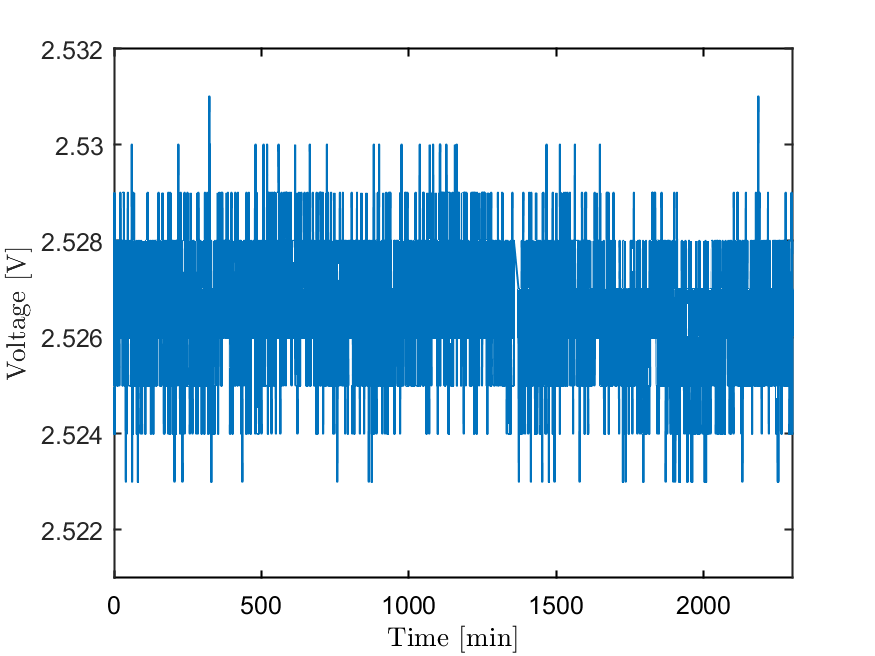
\includegraphics[width=0.65\columnwidth]{Chapter4/images/ROB.png}
    \caption{$V_{out}$ output voltage from one of the DC/DC converters in the \gls{ROB}.}
    \label{fig:ROB}
\end{figure}

The STS-XYTER provides the following information - almost full counter, event missed counter, single event upset counter, the status register, and \gls{ADC} values: VDDM, \gls{CSA} bias, temperature. 

\begin{figure}[!h]
    \centering
    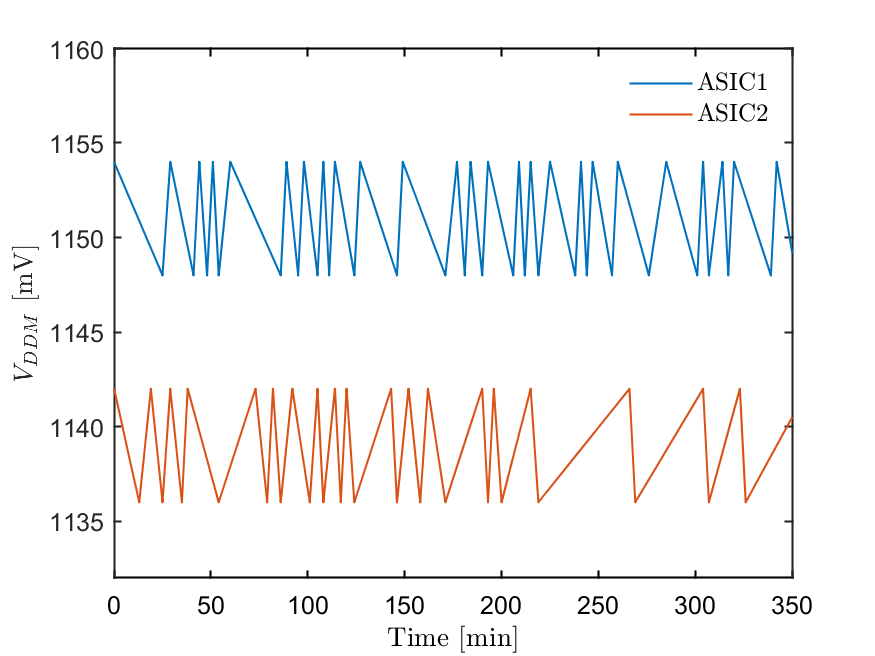
\includegraphics[width=0.65\columnwidth]{Chapter4/images/FEB.png}
    \caption{$V_{ddm}$ readouts from the diagnostic circuits of two ASICs.}
    \label{fig:vddm_first}
\end{figure}
The fluctuations in Figure~\ref{fig:vddm_first} correspond  to the Least Significant Bit of the \gls{ADC}. It's usually defined as
\begin{equation}
    LSB = \frac{V_{REF}}{2^{N}}.
\end{equation}
where the $V_{REF}$ is the reference voltage and N is the number of ADC bits. 
The interface from the \gls{DAQ} chain to the \gls{EPICS}-based system was developed in order to monitor the performance of the \gls{FEE} during numerous tests including the thermal cycling of the detector electronics and \gls{mSTS} setup. 

%\subsection{Parameters of the STS-XYTERv2 ASIC}
%\subsection{GBTX and GBT ASIC monitoring}